% Created 2020-10-21 Wed 21:58
% Intended LaTeX compiler: pdflatex
\documentclass[11pt]{article}
\usepackage[utf8]{inputenc}
\usepackage[T1]{fontenc}
\usepackage{graphicx}
\usepackage{grffile}
\usepackage{longtable}
\usepackage{wrapfig}
\usepackage{rotating}
\usepackage[normalem]{ulem}
\usepackage{amsmath}
\usepackage{textcomp}
\usepackage{amssymb}
\usepackage{capt-of}
\usepackage{hyperref}
\author{adam}
\date{\today}
\title{}
\hypersetup{
 pdfauthor={adam},
 pdftitle={},
 pdfkeywords={},
 pdfsubject={},
 pdfcreator={Emacs 26.3 (Org mode 9.3.8)}, 
 pdflang={English}}
\begin{document}

\tableofcontents

\section{Computer Networks and the Internet}
\label{sec:org264e33f}

\subsection{Internet overview}
\label{sec:org7444823}

\subsubsection{Devices}
\label{sec:orgf6ed8d2}
\begin{itemize}
\item host = end system, runs apps
\end{itemize}

\subsubsection{Communication Links}
\label{sec:org05dde87}
\begin{itemize}
\item fiber, copper, radio, satellite
\end{itemize}

\subsubsection{Packet switches}
\label{sec:org7b5b359}
\begin{itemize}
\item routers and switches
\end{itemize}

\subsection{Service view of the internet}
\label{sec:orgd7567fe}
\subsubsection{Provider of services to apps}
\label{sec:orgab0d384}
\begin{itemize}
\item Web, VoIP, email, games, eCommerce, social net
\end{itemize}

\subsubsection{Programming interface to apps}
\label{sec:org5b2e368}
\begin{itemize}
\item hooks
\item service options (postal)
\end{itemize}


\subsection{Protocols}
\label{sec:org792574f}
\subsubsection{Definition}
\label{sec:org8f95e9b}
A protocol defines the format and the order of messages exchanged
between two or more communicating entitites, as well as the actions
taken on the transmission and/or receipt of a message or other event.

\subsubsection{Required}
\label{sec:org0df08a4}
\begin{itemize}
\item format
\item order of messages
\end{itemize}

\subsection{Network edge}
\label{sec:org9355ca7}
\subsubsection{Access networks}
\label{sec:orgd34cebc}
\begin{itemize}
\item Wired, wireless comms links
\end{itemize}
How does one connect an edge to a router?

\begin{itemize}
\item Frequency division multiplexing
\item Cable network is shared
\item HFC: hybrid fiber coax
\item fiber homes -> ISP router
\item DSL
\item Ethernet

\item WLAN: IEEE\textsubscript{802.11}
\end{itemize}

\subsubsection{Physical media}
\label{sec:org5442da6}
\begin{itemize}
\item Guided (wires)
\item Unguided (radio)
\item Physical link (transmitter, \{\$x\}, receiver)
\item Bit (propagates between)
\end{itemize}


\subsection{Network core}
\label{sec:orgb33dbdf}
\subsubsection{Interconnected routers}
\label{sec:orga43f39e}
\begin{itemize}
\item mesh of interconnected routing packets transmitted at full link
capacity
\end{itemize}

\subsubsection{Delay, loss and throughput in Packet switched networks}
\label{sec:orgd48567e}

\begin{itemize}
\item store and forward
\end{itemize}


\begin{verbatim}

 Source     Router    Destination
|       |____________|       |
|_______|            |_______|

   R_bps               R_bps
\end{verbatim}

L bits per packet

\begin{itemize}
\item End to end delay (assumes zero propagation delay) = 2L / R
\end{itemize}

\subsubsection{Queuing, delay, loss}
\label{sec:orge6a98ff}

\begin{center}
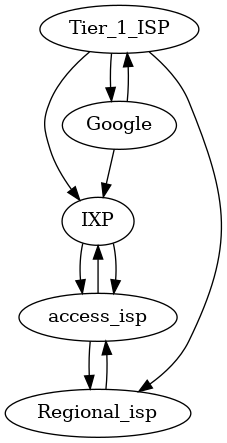
\includegraphics[width=.9\linewidth]{my-diagram.png}
\end{center}

\subsubsection{Sources of delay}
\label{sec:orgb37e2ed}
\begin{itemize}
\item transmission
\item nodal processing
\item queuing
\end{itemize}

\begin{center}
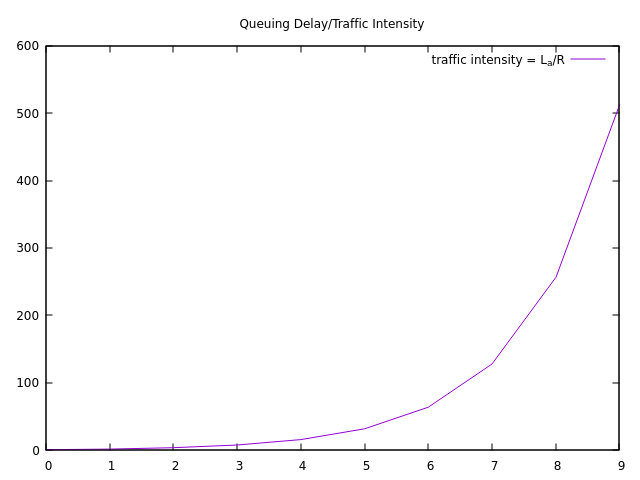
\includegraphics[width=.9\linewidth]{../img/qDelay.png}
\end{center}

\begin{center}
\begin{tabular}{rr}
traffic intensity = L\textsubscript{a}/R & Avg. queuing delay\\
1 & 0\\
2 & 1\\
4 & 2\\
8 & 3\\
16 & 4\\
32 & 5\\
64 & 6\\
128 & 7\\
256 & 8\\
512 & 9\\
\end{tabular}
\end{center}


L\textsubscript{a}/R \textasciitilde{} 0 : avg. q delay small

L\textsubscript{a}/R <= 1 : avg. q delay large

L\textsubscript{a}/R > 1 : more work arriving than can be serviced average delay
infinite

\subsubsection{Packet loss}
\label{sec:orgc55672c}
Buffer has finite capacity 

packet \(\rightarrow\) full queue = dropout


\subsection{Protocol Layers}
\label{sec:org3e37e9a}


\begin{center}
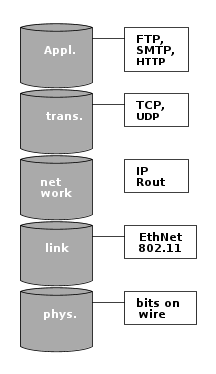
\includegraphics[width=.9\linewidth]{networklayers.png}
\end{center}

\subsubsection{iso/osi Reference Model}
\label{sec:org48ce4a7}

Encapsulation 


\begin{verbatim}

+-------------------+ A |   | A +-------------------+
|               M   |---+   |---+                M  |
|-------------------| T |   | T |-------------------|
|           H_t M   |---+   |---+            H_t M  |
|-------------------| N |   | N |-------------------|
|       H_n H_t M   |---+   |---+        H_n H_t M  |
|-------------------| L |   | L |-------------------|
|    H_l H_n H_t M  |---+   |---+     H_l H_n H_t M |
|-------------------| P |   | P |-------------------|

\end{verbatim}

Source \(\rightarrow\)     Switch \(\rightarrow\)      Router \(\rightarrow\)     Destination 


\subsection{Network Security}
\label{sec:org4346794}

Internet was originally designed to be used be mutual trusting users
attached to a transparent network.

\subsubsection{Malware}
\label{sec:orgd957372}
\begin{itemize}
\item \textbf{Virus}: self-replicating infection by receiving/executing object
(email attachment)
\item \textbf{Worm}: self-replicating infection by passively receiving object
that gets itself executed
\item \textbf{Spyware}: record keystrokes, web sites visited, upload info to
\end{itemize}

Infected host can be enrolled in botnet, used for spam. DDOS attacks.

\begin{itemize}
\item \textbf{DDOS attacks}: make resources unavailable to legitimate traffic by
overwhelming with bogus traffic
\end{itemize}

\subsubsection{Packet "sniffing" \& IP Spoofing}
\label{sec:org78ece56}
\begin{itemize}
\item Broadcast media
\item Promiscuous network interface reads/records all packets passing by
\item Send packet with false source address
\end{itemize}




\section{Application layer}
\label{sec:orga1eef21}

\subsection{Web and HTTP}
\label{sec:orgc616d98}
\subsubsection{Client-Server Architecture}
\label{sec:org2af8313}

\begin{center}
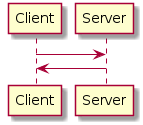
\includegraphics[width=.9\linewidth]{clientserver.png}
\end{center}

\begin{center}
\begin{tabular}{ll}
\textbf{Client} & \textbf{Server}\\
\hline
Communicates with server & Always on host\\
\hline
May be intermittently connected & Permanent IP\\
\hline
May have dynamic IP & Data centers for scaling\\
\hline
Do not communicate directly with each other & \\
\end{tabular}
\end{center}

\subsubsection{Process Communicating}
\label{sec:org2559eee}
Client process initiates comms, server process waits for contact

\subsubsection{Process}
\label{sec:orgabf5fd4}
\begin{itemize}
\item Running within a host
\item Withing same host, two processes communicating using inter-process
communication (defined by OS)
\item Processes in different hosts communicated by exchanging messages
\end{itemize}

\subsubsection{Sockets}
\label{sec:org2315fba}

\begin{verbatim}

    V                  ^
+---v-----+        +---^-----+  
|_V_V_V_V_|        |_V_V_V_V_|

\end{verbatim}

\textbf{Addressing Processes}
\begin{itemize}
\item to receive messages, process must have ID
\item IP = 32 bit
\item identified = IP + Port
\item HTTP server: 80
\item Mail server: 25
\end{itemize}

\textbf{Application Layer Protocol}

Defines:
\begin{itemize}
\item types of messages exchanged (eg: request, response)
\item msg syntax (fields and delineation)
\item msg semantics
\end{itemize}

\subsubsection{Protocols}
\label{sec:org9b1508b}

Open protocols:
\begin{itemize}
\item defined in RFC
\item allows for interoperability
\item eg: http, smtp
\end{itemize}

Proprietary protocols:
\begin{itemize}
\item eg. Skype
\end{itemize}

Transport service for an app
\begin{itemize}
\item 100\% reliable?
\item can tolerate loss
\item low latency
\item multimedia, minimum throughput
\item "elastic apps" whatever throughput
\item encryption data integration
\end{itemize}

Different apps need different architecture to accommodate all user
requirements

\textbf{TCP (Transmission Control Protocol)}
\begin{itemize}
\item Reliable transport send \(\rightarrow\) receive
\item Flow control (doesn't overwhelm receiver)
\item Congestion control (throttle sender when network overloaded)
\item Does not provide: timing, minimum throughput guarantee
\item Connection oriented: setup required between client \& server process
\end{itemize}

\textbf{UDP (User datagram Protocol)}
\begin{itemize}
\item unreliable data transfer between sending and receiving
\item does not provide: reliability, flow control, congestion control,
timing, throughput guarantee, security, or connection setup
\end{itemize}


\begin{center}
\begin{tabular}{lll}
\textbf{App} & \textbf{App layer protocol} & \textbf{underlying transport protocol}\\
\hline
email & SMTP [RFC 2821] & TCP\\
remote terminal access & Telnet [RFC 854] & TCP\\
web & HTTP [RFC 2616] & TCP\\
file transfer & FTP [RFC 959] & TCP\\
streaming & http [rtp 1889] & TCP or UDP\\
VoIP & SIP, RTP, proprietary & TCP or UDP\\
\end{tabular}
\end{center}

\subsubsection{HTTP}
\label{sec:org142d494}
HTTP is a stateless protocol, server maintains no info about previous
client requests
\textbf{uses TCP}
\begin{itemize}
\item client initiates
\item server accepts
\item http messages (application-layer protocol messages) exchanged
between browser (http client) and web server (http server)
\item TCP connection closed
\end{itemize}

\textbf{non-persistent}
\begin{itemize}
\item At most one object sent over TCP connection
\item connection then closed
\item downloading multiple objects required multiple connections
\end{itemize}

\textbf{persistent}
\begin{itemize}
\item multiple objects can be sent over single TCP connection between
client, server
\end{itemize}

\begin{center}
\includegraphics[width=.9\linewidth]{http.png}
\end{center}

\begin{center}
\includegraphics[width=.9\linewidth]{../img/http.png}
\end{center}

\subsubsection{User-server state: Cookies}
\label{sec:org10dd043}
Four components:
\begin{enumerate}
\item Cookie header line of http response message
\item cookie header line in next http request message
\item cookie file kept on user's host, managed by browser
\item back-end database at website
\end{enumerate}

\textbf{uses}
\begin{itemize}
\item authentication
\item shop cart
\item recommend
\item user session state (web-mail)
\end{itemize}

\textbf{cookies and privacy}
\begin{itemize}
\item permit site to learn about users
\end{itemize}

\subsubsection{Web caches (proxy server)}
\label{sec:orgc39c438}
\begin{itemize}
\item acts as both client and server
\item typically installed by ISP (uni, company, residential)
\item reduce response time
\item reduce traffic on access link
\end{itemize}

\subsubsection{conditional GET}
\label{sec:orgc928a02}

\begin{itemize}
\item \textbf{goal}: don't send object if cache has up to date cached version
\item \textbf{cache}: specify date of cached copy in http request
\item \textbf{server}: response contains no object if cached copy up to date
\end{itemize}

\subsection{FTP}
\label{sec:org4788858}
File Transfer Protocol 

\begin{itemize}
\item to/from remote host
\item client/server model
\begin{itemize}
\item initiated by client
\item server: remote host
\end{itemize}
\item Ftp: RFC 959
\item Ftp server: port 21
\end{itemize}

\subsection{Electronic mail: SMTP, POP3, IMAP}
\label{sec:orgb5d3da5}
\begin{itemize}
\item User agent
\item mail server
\item SMTP
\end{itemize}

\textbf{Uses TCP on port 25}
Three phases:
\begin{itemize}
\item handshaking
\item Transfer
\item closure
\end{itemize}

\subsubsection{POP3}
\label{sec:org36ff020}
\begin{itemize}
\item download \& delete
\item cannot re-read file after client change
\item stateless across sessions
\item download-and-keep copies and different clients
\end{itemize}

\subsubsection{IMAP}
\label{sec:org3960252}
\begin{itemize}
\item keeps messages in one place:server
\item allows user to organize messages in folders
\item keeps user state across sessions:
\begin{itemize}
\item names of folders and mappings between message IDs and folder name
\end{itemize}
\end{itemize}

\subsection{DNS}
\label{sec:org7ac1217}
Domain Name System

\begin{itemize}
\item Names map IP to readable format
\item Distributed database implemented in hierarchy of many name servers
\item application-layer protocol: hosts, name servers communicate to
resolve names (address/name translation)
\begin{itemize}
\item Note: core Internet function implemented as application-layer
protocol complexity at network's edge
\end{itemize}

\item \textbf{Root DNS Servers} over 400 worldwide (2016 numbers)
\item \textbf{Top-level domain (TLD) servers} for each of \{com, org, ned, edu,
gov, ie, at, jp, etc) there is a server or server cluster
\item \textbf{Authoritative DNS servers} publicly accessible records that map the
names of the host companies to IP addresses
\end{itemize}


\subsubsection{DNS Services}
\label{sec:orgd7134d1}
\begin{itemize}
\item Host-name to IP address translation
\item host aliasing
\begin{itemize}
\item canonical alias names
\end{itemize}
\item mail server aliasing
\item load distribution 
\begin{itemize}
\item replicated web servers: many IP addresses correspond to one name
\end{itemize}
\end{itemize}

\textbf{Why not centralize DNS?}
\begin{itemize}
\item single point of failure
\item traffic volume
\item distant centralized database
\item maintenance
\item doesn't scale
\end{itemize}

\subsubsection{DNS Records}
\label{sec:org45d1be8}

DNS: distributed db storing resource records (RR) 

RR Format: (name, value, type, ttl)

\textbf{type=A}
\begin{itemize}
\item name is host-name
\item value is IP
\end{itemize}

\textbf{type=NS}
\begin{itemize}
\item name is domain
\item value is host-name of authoritative name server for this domain
\end{itemize}

\textbf{type=CNAME}
\begin{itemize}
\item name is alias for some "canonical" real name
\item www.ibm.com
\begin{itemize}
\item servereast.backup2.ibm.com
\item value is canonical name
\end{itemize}
\end{itemize}

\textbf{type=MX}
\begin{itemize}
\item value is name of mail server associated with name
\end{itemize}


\subsubsection{Attacking DNS}
\label{sec:org8a3f683}

\textbf{DDoS attacks}
\begin{itemize}
\item Bombard servers with traffic
\begin{itemize}
\item Not successful to date
\item traffic filtered
\item local DNS servers cache IPs of TLD servers, allowing root server
bypass
\end{itemize}
\item Bombard TLD (top level domain) servers
\begin{itemize}
\item potentially more dangerous
\end{itemize}
\end{itemize}

\textbf{Redirect attacks}
\begin{itemize}
\item man in the middle attacks
\begin{itemize}
\item intercept queries
\end{itemize}
\item DNS poisoning
\begin{itemize}
\item send bogus replies to DNS server, which caches
\end{itemize}
\end{itemize}

\textbf{Exploit DNS for DDoS}
\begin{itemize}
\item send queries with spoofed source address: target IP
\item requires amplification
\end{itemize}

\subsection{Principles of network applications}
\label{sec:orged38310}
\subsubsection{Server/client}
\label{sec:orgad126af}
\begin{itemize}
\item send one copy F/u\textsubscript{S}
\item send N copes NF/u\textsubscript{s}
\end{itemize}

Client must download file copy
\begin{itemize}
\item d\textsubscript{min} = min client dl rate
\item min client download time: F/d\textsubscript{min}
\end{itemize}

\textbf{Distribution time}

D\textsubscript{c}-s > mac\{NF/u\textsubscript{s} , F/d\textsubscript{min}\}

\subsubsection{P2P}
\label{sec:org29154e4}

Max upload rate:  u\textsubscript{s} + \(\Sigma\) u\textsubscript{i}

distribution time (\emph{increases linearly in N}):

D\textsubscript{p2p} > max \{ F/u\textsubscript{s}, F/d\textsubscript{min}, NF/(u\textsubscript{s} + \(\Sigma\) u\textsubscript{i}) \}





\subsection{P2P Apps}
\label{sec:org7dc2c17}
Commonly used to distribute software

Distributed hash table (DHT)

DHT: a distributed P2P database


\section{Transport Layer}
\label{sec:org165c73b}

\subsection{Transport Services \& Protocols}
\label{sec:orgc50c391}
\begin{itemize}
\item Provide logical communication between app processes running on
different hosts
\item Transport protocols run in and systems
\begin{itemize}
\item Send side: breaks app messages into segments, passes to network layer
\item receiver side: reassemble segments into messages, passes to app
layer
\end{itemize}
\item More than one transport protocol available to apps
\begin{itemize}
\item Internet: TCP \& UDP
\end{itemize}
\end{itemize}

\subsection{Multiplexing and Demultiplexing}
\label{sec:orga9e503a}
\begin{itemize}
\item Multiplexing at sender: handle data from multiple sockets, add
transport  header (later used for demultiplexing)
\item Demultiplexing at receiver: use header info to deliver received
segments to correct socket
\end{itemize}

\subsubsection{Port}
\label{sec:org156248b}
Simply a number used by a particular software to identify its data
coming from the internet

\subsubsection{Socket}
\label{sec:org4cc4a81}
IP Address + Port num. Used by another computer to send data to
software on a particular machine 
\begin{itemize}
\item IP = Machine
\item Port = Software
\end{itemize}


\break

\subsection{Demultiplexing}
\label{sec:org592306a}

\begin{itemize}
\item Host receives IP datagrams
\begin{itemize}
\item Each datagram has source IP address, destination IP address
\item Each datagram carries one transport-layer segment
\end{itemize}
\item Host uses IP address \& port numbers to direct segment to appropriate
socket
\end{itemize}

\begin{verbatim}

<-----------32 bits--------->
+-------------+-------------+
| src port #  | dest port # |
|_____________|_____________|
|                           |
|     other header fields   |
|___________________________|
|                           |
|       application data    |   
|       payload             |
|___________________________|

\end{verbatim}
\captionof{figure}{TCP/UDP segment format}

\subsubsection{Connection-less Dmuxing}
\label{sec:org6d00ac7}
When host receives UDP segment:
\begin{itemize}
\item checks destination port number in segment
\item directs UDP segment to socket with that port number
\end{itemize}

IP datagrams with some destination port number, but different source IP
and/or source port numbers will be directed to same socket at destination.

\subsubsection{Connection-oriented Dmux}
\label{sec:org33b788d}
TCP socket identified by 4-tuple:
\begin{itemize}
\item Source IP address
\item Source port number
\item Destination IP address
\item Dest port number
\end{itemize}

Server host may support many simultaneous TCP sockets: each socket
identified by its own 4-tuple.Web servers have different sockets for
each connecting client, non persistent http will have different socket
for each request

\subsection{Connection-less Transport UDP}
\label{sec:org2774d5e}
\begin{itemize}
\item No handshaking between UDP, sender, receiver
\item each UDP segment handled independently of others
\end{itemize}

UDP uses:
\begin{itemize}
\item streaming multimedia apps (loss tolerant, rate sensitive)
\item DNS
\item best effort service
\end{itemize}

UDP segments may be
\begin{itemize}
\item lost
\item delivered out-of-order to app
\end{itemize}


\begin{verbatim}

<-----------32 bits--------->
+-------------+-------------+
| src port #  | dest port # |
|_____________|_____________|
| length      | checksum    |
|_____________|_____________|
|                           |
|     other header fields   |
|___________________________|
|                           |
|       application data    |   
|       payload             |
|___________________________|

\end{verbatim}
\captionof{figure}{UDP segment format}

\subsubsection{Why UDP?}
\label{sec:orgfcea9e9}
\begin{itemize}
\item No connection establishment (which can add delay)
\item Simple: no connection state at sender, receiver
\item Small header size
\item No congestion control: UDP can blast away as fast as desired
\end{itemize}

\subsection{Principles of Reliable Data Transfer}
\label{sec:org3a78a62}

\begin{figure}[htbp]
\centering
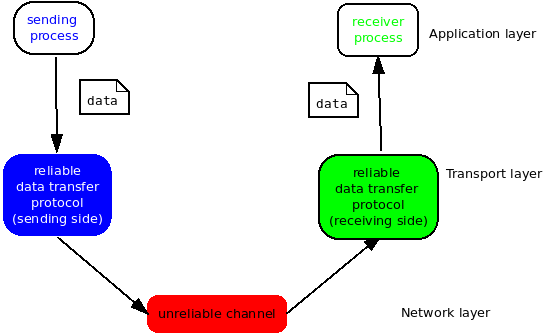
\includegraphics[width=.9\linewidth]{../img/RDT.png}
\caption{Reliable Data Transfer (RDT)}
\end{figure}

\subsubsection{RDT: Getting Started}
\label{sec:org57d9635}

Relies on four functions

\begin{verbatim}

rdt_send()

deliver_data()

udt_send()

rdt_rcv()

\end{verbatim}


\subsubsection{Dependency between event \& state}
\label{sec:orgc661cb0}

\begin{figure}[htbp]
\centering
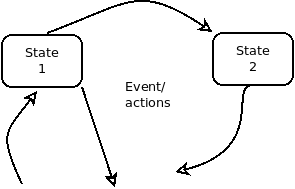
\includegraphics[width=.9\linewidth]{../img/eventStateDependency.png}
\caption{Event -><- State dependency}
\end{figure}


\subsubsection{RDT 1.0}
\label{sec:orgf1a4c0b}
Reliable data transfer over a reliable channel. Underlying channel is
perfectly reliable
\begin{itemize}
\item no bit errors
\item no loss of packets
\end{itemize}

Separate FSMs for sender, receiver:
\begin{itemize}
\item sender sends data into underlying channel
\item receiver reads data from underlying channel
\end{itemize}

\textbf{a. rdt1.0 sending side}

\begin{center}
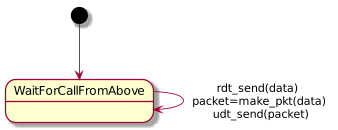
\includegraphics[width=.9\linewidth]{rdt1.0senderFSM.png}
\end{center}

\textbf{b. rdt1.0: receiving side}
\begin{center}
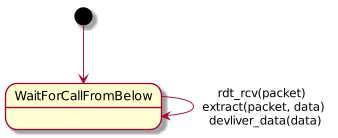
\includegraphics[width=.9\linewidth]{rdt1.0receiverFSM.png}
\end{center}


\subsubsection{RDT 2.0}
\label{sec:orgee901b5}
Channel with bit errors: underlying channel may flip bits in packet
\begin{itemize}
\item checksum to detect bit
\end{itemize}

\textbf{Question}: How to recover from errors?

\begin{itemize}
\item Acknowledgements (ACKs): receiver explicitly tells sender that pkt
received OK
\item Negative acknowledgements (NAKs): receiver explicitly tells sender
that pkt had errors
\item Sender re-transmits pkt on receipt of NAK
\end{itemize}

\textbf{FATAL FLAW}
ACK/NAK can be corrupted
\begin{itemize}
\item sender doesn't know what happened at receiver
\item can't just re-transmit possible duplicate
\end{itemize}

Handling duplicates:
\begin{itemize}
\item Sender retransmits current pkt if ACK/NAK corrupted
\item Sender adds sequence number to each pkt
\item Receiver discards (doesn't deliver up) duplicate pkt
\end{itemize}

Stop and wait:
\begin{itemize}
\item sender sends one packet, then waits for receiver to respond
\end{itemize}


\textbf{a. rdt2.0 sending side}

\begin{center}
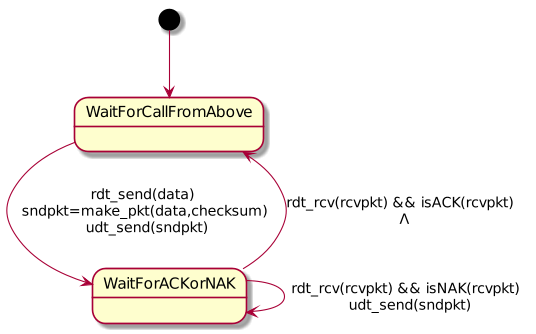
\includegraphics[width=.9\linewidth]{rdt2.0senderFSM.png}
\end{center}

\textbf{a. rdt2.0 receiving side}

\begin{center}
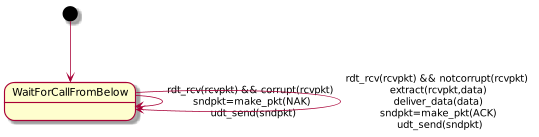
\includegraphics[width=.9\linewidth]{rdt2.0receivingFSM.png}
\end{center}




\subsubsection{RDT 2.1}
\label{sec:org8c2de2f}
Sender:
\begin{itemize}
\item Seq number added to pkt
\item Two sequence numbers (0,1) will suffice
\item Must check if ACK/NAK corrupted
\item Twice as many states
\begin{itemize}
\item states must "remember" whether "expected" pkt should have sequence
number of 0 or 1
\end{itemize}
\end{itemize}

Receiver: 
\begin{itemize}
\item Must check if received packet is duplicate
\begin{itemize}
\item State indicates whether 0 or 1 expected pkt sequence number
\end{itemize}
\end{itemize}

Note: receiver can not(!) know if its last ACK/NAK received okay at
sender 

\subsubsection{RDT 2.2: A NAK-free protocol}
\label{sec:orgbb0225a}

+Same functionality as \textbf{RDT 2.1}, using ACKs only 
\begin{itemize}
\item Instead of NAK, receiver sends ACK for last pkt received OK
\begin{itemize}
\item receiver must explicitly include sequence number of packet being
ACKed
\end{itemize}
\item Duplicate ACK at sender results in same action as NAK: re-transmit
current pkt
\end{itemize}

\subsubsection{RDT 3.0: Channels with errors and loss}
\label{sec:orge09f5b9}

\textbf{New assumption}: underlying channel can also lose packets (data,
ACKs)
\begin{itemize}
\item checksum, sequence number, ACKs, transmission will be of help
\ldots{} but not enough
\end{itemize}

\textbf{Approach}: Sender waits reasonable amount of time for ACK
\begin{itemize}
\item retransmits if no ACK received in this time
\item if pkt (or ACK) just delayed (not lost)
\begin{itemize}
\item re-transmission will be duplicate, but sequence numbers already
handles this
\item receiver must specific sequence number of pkt being ACK
\end{itemize}
\item Requires countdown timer
\end{itemize}



\begin{center}
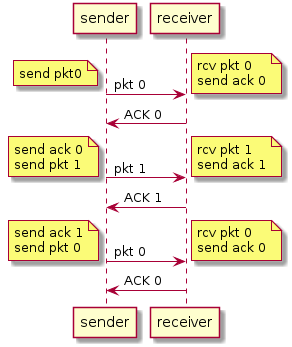
\includegraphics[width=.9\linewidth]{RDT3.0.png}
\end{center}



\subsection{Pipelined Protocols}
\label{sec:orga2e8ec4}

\begin{center}
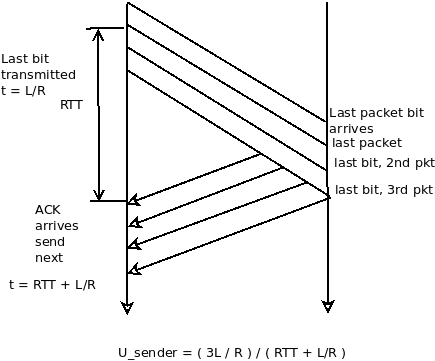
\includegraphics[width=.9\linewidth]{../img/pipelined_protocols.png}
\end{center}

\subsubsection{Got-back-N}
\label{sec:org1f01267}
\begin{itemize}
\item Sender can have up to N unacked packets in a pipeline
\item Receiver only sends cumulative ack
\begin{itemize}
\item doesn't ack packet if there is a gap
\end{itemize}
\item Sender has a timer for oldest unacked packet
\begin{itemize}
\item when timer expires, re-transmit all unacked packets
\end{itemize}
\end{itemize}

Packets also carry status tag, sending happens through a window

\subsubsection{Selective repeat}
\label{sec:orgbbc4ec4}
\begin{itemize}
\item Sender can have up to N unacked packets in a pipeline
\item Receiver sends individual ack for each packet
\item Sender maintains timer for each packet
\item When timer expires, re-transmit only that unacked packet
\end{itemize}


Individual acknowledgements happen on a per packet basis

\subsection{TCP}
\label{sec:org10f80b6}
\subsubsection{Overview}
\label{sec:org49bf41f}

A TCP "connection" is not an end-to-end switched circuit. It exists
rather as a logical connection, where common state resides only in the
TCPs in the two communicating end systems. None of the intermediate
network or link layer elements retain any information about the
connection and are in fact "oblivious" that even one exists.
"Multicasting" is not possible as the connection needs to be point to
point as a \textbf{full duplex service}.

\begin{itemize}
\item RFCs: 737, 1122, 1323, 2018, 2581
\item Point to point (\textbf{connection-oriented})
\begin{itemize}
\item one sender, one receiver
\end{itemize}
\end{itemize}

\subsubsection{TCP seq Number Acks}
\label{sec:orgab166e2}
Sequence numbers:
\begin{itemize}
\item byte stream "number" of first byte in segment's data
\end{itemize}

Acknowledgements:
\begin{itemize}
\item Seq number of next byte expected from other side
\item cumulative ACK
\end{itemize}

\begin{center}
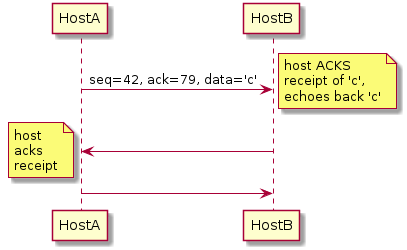
\includegraphics[width=.9\linewidth]{telnetEG.png}
\end{center}



\subsubsection{Round Trip Time, Timeout}
\label{sec:org0c640bb}
\textbf{Q Set?}
\begin{itemize}
\item longer than RTT
\begin{itemize}
\item RTT varies
\end{itemize}
\item too short: premature timeout, unnecessary transmission
\item too long: show reaction to segment loss
\end{itemize}

\textbf{Estimate ?}
\begin{itemize}
\item Sample RTT: measured time from segment transmission until ACK
receipt 
\begin{itemize}
\item ignore transmissions
\end{itemize}
\item sample RTT will vary, want RTT smoother
\begin{itemize}
\item average several recent measurements
\end{itemize}
\end{itemize}


Estimated RTT = ( 1 - \(\alpha\) ) * EstmiatedRTT + \(\alpha\) * SampleRTT

\subsubsection{Re-transmission}
\label{sec:orgbcb6ea2}
\textbf{Cumulative Acknowledgement} indicates that all packets with a sequence


\textbf{TCP ACK Generation}

\begin{center}
\begin{tabular}{ll}
\hline
event receiver & TCT receiver action\\
\hline
in order all up to & delayed ACk, wait up to 500ms for\\
expected seq \# acked & for next segment, if none send ack\\
\hline
arrived in order & immediately send single\\
one other seq ack pending & cumulative ack, acking both\\
 & in order segs\\
\hline
out of order GAP detected & immediately send duplicate ACK\\
 & with seq \# of expected byte\\
\hline
missing segment arrives & immediate ACK sent\\
\hline
\end{tabular}
\end{center}


\textbf{Fast Re-transmit}

In the event of a lost segment in the course of a transfer, this can
lead to a backlog of duplicate ACKs. In order to overcome this problem,
if the sender receives three duplicates ACKs for a segment, it
retransmits this particular segment using \textbf{fast re-transmit} before the
segment's timer has expired.

\begin{verbatim}

event: ACK received, with ACK field value of y 
	if(y > SendBase) {
	    sendBase = y
	    if(there are currently any not yet acknowledged segments)
	       start timer
	}

\end{verbatim}

\subsubsection{Flow Control}
\label{sec:org6efb633}
\begin{itemize}
\item Receiver controls sender, so sender won't overflow receiver's buffer
by sending too much, too fast
\item Receiver advertises window space into header of request ack
\end{itemize}

\subsubsection{Connection Management}
\label{sec:org94138e8}
\begin{itemize}
\item TCP: 3 way handshakes
\end{itemize}

\begin{center}
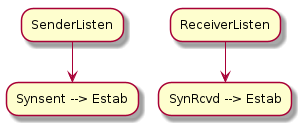
\includegraphics[width=.9\linewidth]{connectionManagement.png}
\end{center}


\begin{center}
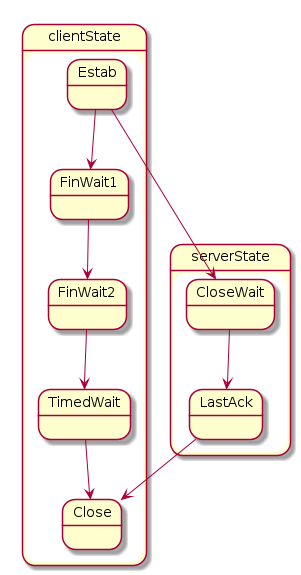
\includegraphics[width=.9\linewidth]{TCPclosing.png}
\end{center}

\subsubsection{Principles of Congestion Control}
\label{sec:orga5f74be}
otherwise known as traffic ;-)

Another cost of congestion: when packet dropped, any "upstream
transmission capacity used for that packet was wasted!"

\begin{itemize}
\item Additive increase multiplicative decrease (AIMD)
\end{itemize}

\section{Network Layer}
\label{sec:org428f4d8}

\subsection{Data Plane}
\label{sec:orga56c44b}
\begin{itemize}
\item Transport segments from sending to receiving host
\item On send side encapsulates segments into datagrams
\item On receiving side, delivers segments to transport layer
\item Router examines header Fields in all IP datagrams passing through it
\end{itemize}

\subsubsection{Forwarding}
\label{sec:org553016d}
\begin{itemize}
\item \textbf{defn} Move packets from routers' input to appropriate router output
\item \textbf{analogy} planning a trip from source to destination
\end{itemize}

\subsubsection{Routing}
\label{sec:org9b61dcc}
\begin{itemize}
\item \textbf{defn} determine route taken by packets from sources to destination
\item \textbf{analogy} getting through a single intersection
\end{itemize}

\subsection{Control Plane}
\label{sec:org7ddc2a8}

\begin{verbatim}

	       { routing algorithm } -> determines end to end 
					path through network

Control plane -> software-defined networking

..............................................

Data plane       local forwarding table
	     _______________________________
	      header value | output link 
	     --------------|--------------
		   0100    | 3
		   0101    | 2 
		   0111    | 2 
		   1001    | 1

\end{verbatim}


\subsection{Network Services Model}
\label{sec:org1adb0bf}


\begin{center}
\begin{tabular}{lllllll}
Net Arch & Model & Bandwidth & Loss & Order & Timing & Congestion feeback\\
\hline
internet & best effort & none & no & no & no & no (inferred via loss)\\
\hline
ATM & CBR & const rate & yes & yes & yes & no congestion\\
\hline
ATM & VBR & const rate & yes & yes & yes & no congestion\\
\hline
ATM & ABR & grntd. min & no & yes & no & yes\\
\hline
ATM & UBR & none & no & yes & no & no\\
\hline
\end{tabular}
\end{center}


\subsubsection{Possible service provisions}
\label{sec:orgc057f03}
\begin{itemize}
\item guaranteed delivery: packet sent by host will eventually arrive at
destination host
\item guaranteed delivery with bounded delay: e.g. within 100msec
\item In-order packet delivery: guarantees that packets arrive at
destination in the order that they were sent
\item guaranteed
\end{itemize}

\subsection{Virtual circuit \& datagram Network}
\label{sec:org557c816}
\begin{itemize}
\item Datagram network provides network-layer connectionless service
\item virtual-circuit network provides network-layer connection service
\item analogous to TCP/UDP connection-oriented/conectionless transport
layer services, but:
\begin{itemize}
\item Service: host-to-host
\item No choice: network provides one or the other
\item Implmentation: in network core
\end{itemize}
\end{itemize}

\subsubsection{Virtual circuits}
\label{sec:org67541dd}
\begin{itemize}
\item "Source-to-destination path behaves much like telephone circuit"
\begin{itemize}
\item Performance-wise
\item Network actions along source-to-dest path
\end{itemize}
\item Call setup, teardown for each call before data can flow
\item Each packet carries VC identifier (not destination host address)
\item Every router on source-dest path maintains "state" for each passing connection
\item Link, router resources (bandwidth, buffers) may be allocated to VC
(dedicated resources = predictable results)
\end{itemize}


\subsubsection{Datagram forwarding table}
\label{sec:org51b5d35}


\begin{center}
\begin{tabular}{r}
local forwarding table\\
\hline
header value & output lnk\\
\hline
1 & 4\\
2 & 2\\
3 & 2\\
4 & 1\\
\end{tabular}
\end{center}


\begin{itemize}
\item 4 billion IP addresses so rather than list individual destination
addresses, list range of addresses (aggregate table entries)
\end{itemize}

\subsection{Internet (datagram)}
\label{sec:orgd2ee5f1}
\begin{itemize}
\item Data exchange amoung computers
\begin{itemize}
\item "Elastic" service, no strct timing requirements
\end{itemize}
\item Many link types 
\begin{itemize}
\item different characteristics
\item uniform service difficult
\end{itemize}
\item "Smart" end systems (computers)
\begin{itemize}
\item can adapt, perform control, error recovery
\item simple inside network, complexity at "edge"
\end{itemize}
\end{itemize}

\subsection{ATM (VC)}
\label{sec:org5e700a3}
\begin{itemize}
\item Evolved from telephony
\item Human conversation:
\begin{itemize}
\item Strict timing, reliability requirements
\item Need for guaranteed service
\end{itemize}
\item "Dumb" end systems
\begin{itemize}
\item Telephones
\item Complexity inside network
\end{itemize}
\end{itemize}


\subsection{Router Architecture Overview}
\label{sec:org09a56f2}

\begin{center}
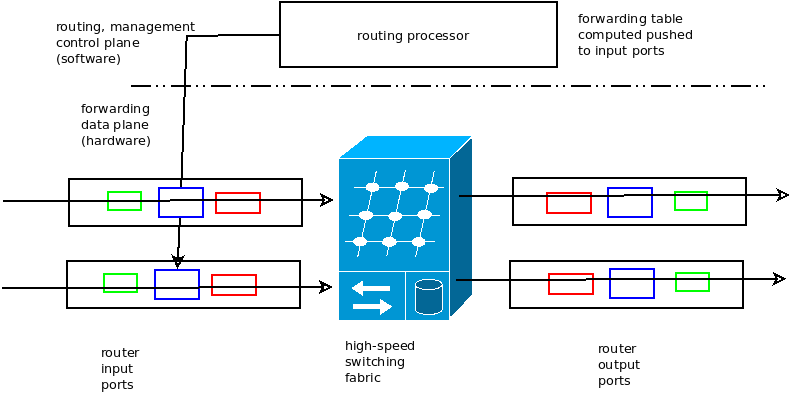
\includegraphics[width=.9\linewidth]{../img/routerArchitecture.png}
\end{center}

Two key functions:
\begin{itemize}
\item Forwarding datagrams from incoming to outgoing link
\item Run routing algorithms/protocol (RIP, OSPF, BGP)
\end{itemize}


\subsubsection{Input port functions}
\label{sec:orgd123eea}

\begin{center}
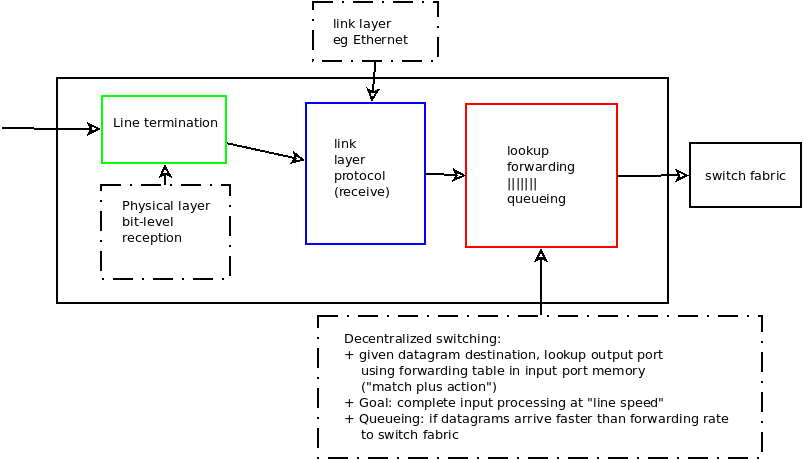
\includegraphics[width=.9\linewidth]{../img/inputPortFunctions.png}
\end{center}

\subsubsection{Head-of-the-line (HOC) blocking}
\label{sec:orga478ca5}

\begin{center}
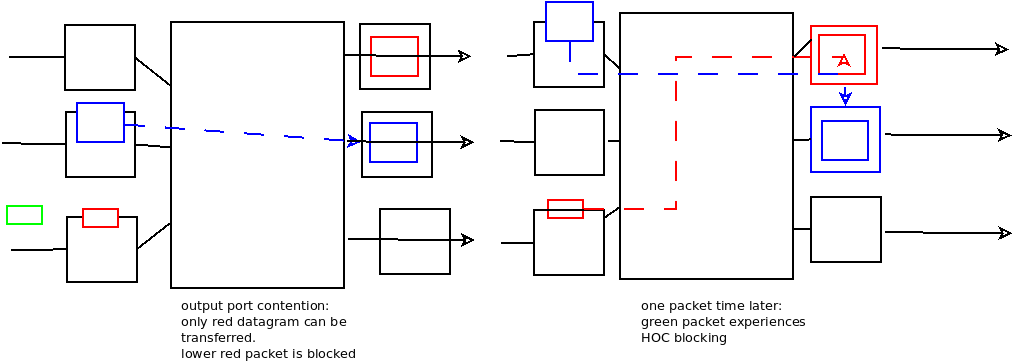
\includegraphics[width=.9\linewidth]{../img/hocBlocking.png}
\end{center}

\subsubsection{Switching Fabric}
\label{sec:org7df2c79}

\begin{center}
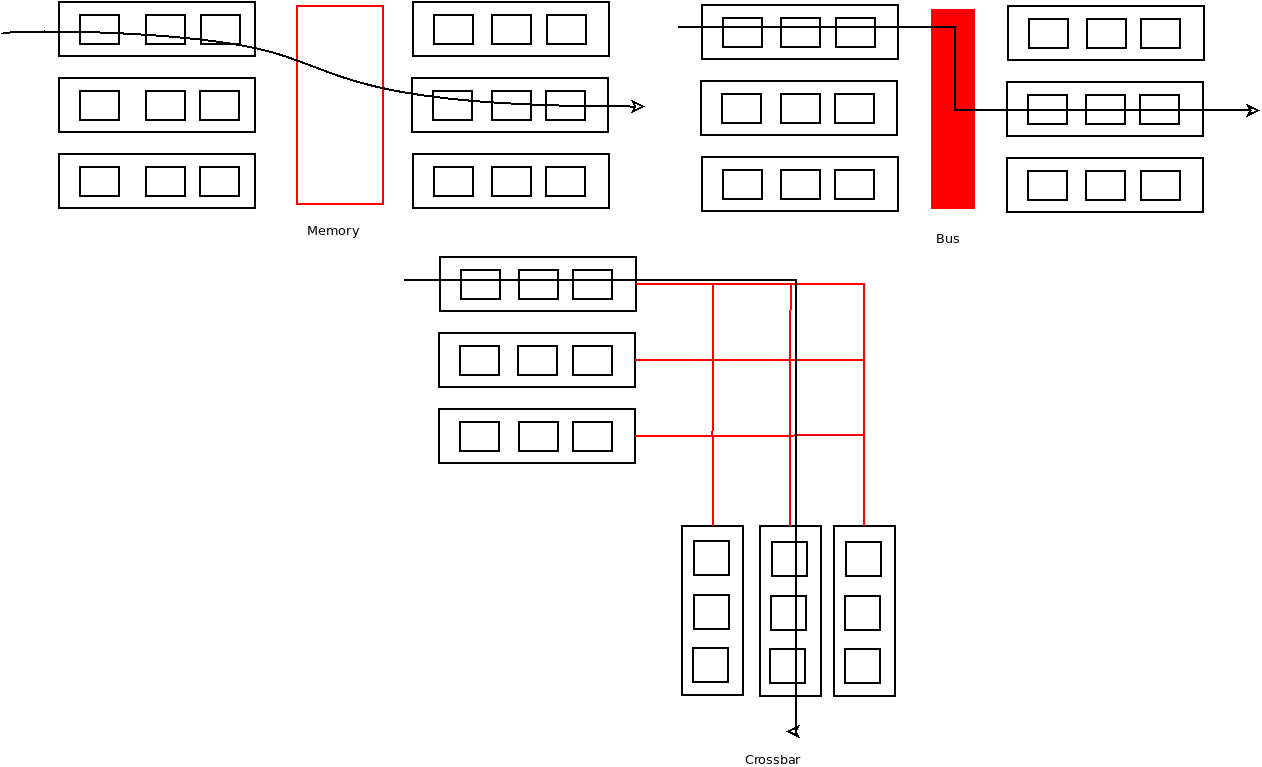
\includegraphics[width=.9\linewidth]{../img/switchingFabric.png}
\end{center}

\subsubsection{Output Ports}
\label{sec:org547569e}

\begin{center}
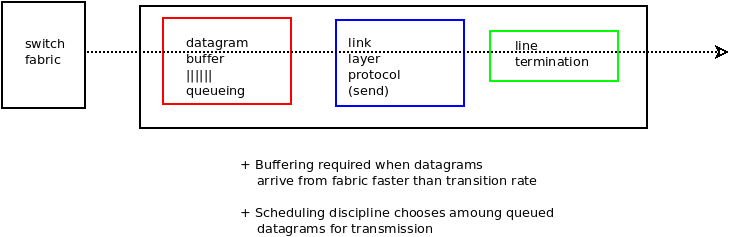
\includegraphics[width=.9\linewidth]{../img/outputPorts.png}
\end{center}

\subsection{IP Layer Protocol}
\label{sec:org8a5c410}

\begin{center}
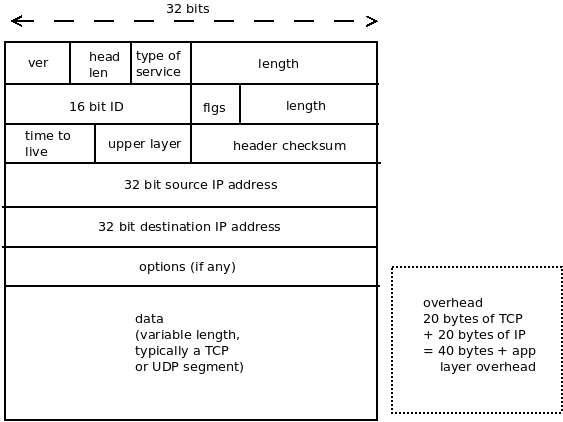
\includegraphics[width=.9\linewidth]{../img/ipLayerProtocol.png}
\end{center}


\subsection{IP Fragmentation, Reassembly}
\label{sec:org7234bc9}

Large IP datagram divided ("fragmented") within net
\begin{itemize}
\item One datagram decomes several datagrams
\item Reassaembled only at final destination
\item IP header bits used to identify, order related fragments
\end{itemize}

\subsection{IP Addressing}
\label{sec:org079cf57}
\begin{itemize}
\item IP Address: 32 bit identifier for host, router interface
\item Interface: connection between host/router and physical link
\begin{itemize}
\item Routers typcially have multiple interfaces
\item host typically has one or two interfaces (e.g. wired Ethernet,
wireless 802.11)
\end{itemize}
\item IP address associated with each interface
\end{itemize}

\subsection{Subnets}
\label{sec:org645fe30}

\begin{center}
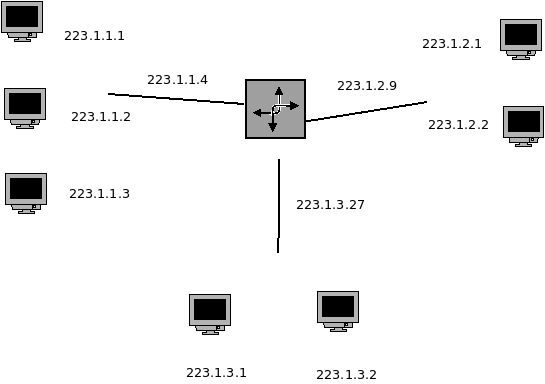
\includegraphics[width=.9\linewidth]{../img/subnetsIP.png}
\end{center}

\begin{itemize}
\item Subnet? 
\begin{itemize}
\item Device interfaces with same subnet port of IP address
\item Can physically reach out to each other without intervening router
\end{itemize}
\item IP Address 
\begin{itemize}
\item Subnet port: high order bits
\item host port: low order bits
\end{itemize}
\end{itemize}

\subsubsection{Bit distribution and max num Computers}
\label{sec:orgb3169d9}

On the subnet: 23.1.1.0/24 the last 8 bits are used to ID the computer 

2\textsuperscript{8} = 256 
0 => ID Network
255 => ID Broadcast

Max of 254 computers on a subnet

\subsubsection{CIDR (RFC 1918)}
\label{sec:orgaacbf6b}
Classless InterDomainRouting
\begin{itemize}
\item Subnet portion of address of arbitrary length
\item Address format \emph{a.b.c.d/c} , where \emph{x} is the number of bits in
subnet portion of address
\end{itemize}

\begin{center}
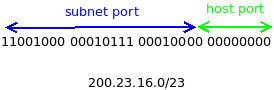
\includegraphics[width=.9\linewidth]{../img/cidr.png}
\end{center}


\subsection{How to get IP}
\label{sec:orgb272ce1}

\subsubsection{Host}
\label{sec:org60dfcfc}
\begin{itemize}
\item can hard code via system files 
\begin{itemize}
\item windows: control-panel \(\rightarrow\) network \(\rightarrow\)
configuration \(\rightarrow\) tcp/ip \(\rightarrow\) properties
\item unix: /etc/rc.config
\end{itemize}

\item Assigned by DHCP (Dynamic Host Configuration Protocol)
\begin{itemize}
\item "Plug \& Play"
\end{itemize}
\end{itemize}

DHCP can return more than just allocated IP address on subnet:
\begin{itemize}
\item Address of first-hop router for client
\item name and IP address of DNS server
\item Network mask (indicating network versus host portion of address)
\end{itemize}


\subsubsection{Network}
\label{sec:org17df893}
Q. How does network get subnet part of IP address?

A. Gets allocated portion of its provider's ISP address space

Basically, the ISP's IP is chunked into a large enough block that
anything being sent through the internet will be associated with a
specific "IP address range", i.e. the whole 32 bits will note have to
be constrantly re-read

ISP receives block from 

ICANN (icann.org)
\begin{itemize}
\item allocated addresses
\item manages DNS
\item assignes domain names, resolves disputes
\end{itemize}

\subsection{NAT: Network Address Translation}
\label{sec:org1b41b26}

\begin{itemize}
\item Problem: not enough IP addresses
\item Private internet addresses
\end{itemize}

\begin{center}
\begin{tabular}{ll}
\hline
class & block\\
\hline
A & 10.0.0/8\\
B & 172.16.0.0/12\\
C & 192.168.0.9/16\\
\hline
\end{tabular}
\end{center}

Basically, a router will map a pricate IP to a public one

\begin{center}
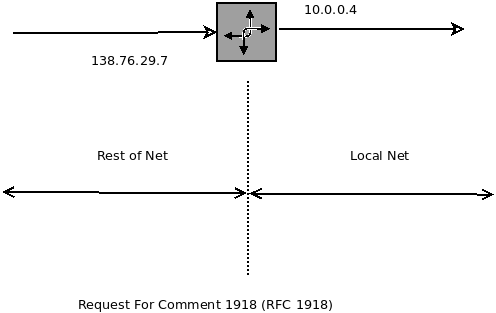
\includegraphics[width=.9\linewidth]{../img/routerIPMap.png}
\end{center}

Local network uses just one IP address as far as the outside world is
concerned:
\begin{itemize}
\item Range of addresses not needed from ISP just one IP address for all devices
\item Can change addresses of devices in local network without notifying
outside world
\item can change ISP without changing addresses of devices in local network
\item Devices inside local net not explicitly addressable, visible by
outside world (a security plus)
\end{itemize}

\subsection{Routing Algorithms}
\label{sec:org4b6ee0c}
\begin{itemize}
\item Algorithm responsible for maintaining the path that the datagram
travels through the network
\item Forwarding takes packet coming into incoming port, processes it,
does the lookup on the destination and forwards it to the router
\end{itemize}

\subsubsection{Graph Abstraction}
\label{sec:org68f8922}

\begin{center}
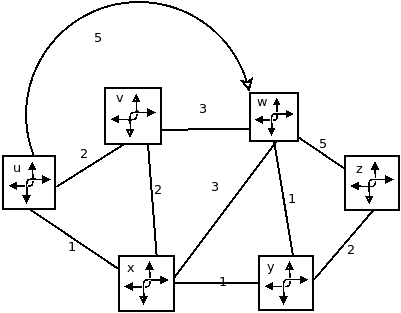
\includegraphics[width=.9\linewidth]{../img/graphAbstraction.png}
\end{center}

\begin{itemize}
\item C( x, x\textsuperscript{1} ) = const of link ( x, x\textsuperscript{1} ) e.g.: c( w, z ) = 5
\item cost could always be 1, or inversely related to bandwidth, or
inversely related to congestion
\item Cost of path ( x\textsubscript{1} , x\textsubscript{2} , \ldots{} , x\textsubscript{p} ) = c( x\textsubscript{1} , x\textsubscript{2} ) + c( x\textsubscript{2} ,
x\textsubscript{3} ) + \ldots{} + c( x\textsubscript{p}-1 , x\textsubscript{p} )

\item Key question: what is the least-cost path between u and z?

\item Routing algorithm: algorithm that finds that least cost path
\end{itemize}

\subsubsection{Routing Algorithm Classification}
\label{sec:org5f83d4c}
Global or decentralized information?

\textbf{Global:}
\begin{itemize}
\item All routers have complete topology, link cost info
\item "Link state" algorithms
\end{itemize}

\textbf{Decentralized}
\begin{itemize}
\item Router knows physically-connected neighbors, link cost to neighbors
\item Iterative process of computation, exchange of info with neighbors
\item "Distance vector" algorithms
\end{itemize}

\textbf{Q.} \emph{Static or Dynamic?}

\textbf{Static}
\begin{itemize}
\item Routes change slowly over time
\end{itemize}

\textbf{Dynamic}
\begin{itemize}
\item Routes change more quickly
\begin{itemize}
\item Periodic update in response to link cost changes
\item Global
\item Decentralized
\item Static
\item Dynamic
\end{itemize}
\end{itemize}

\subsubsection{Link State: Dijkstra's Algorithm}
\label{sec:org13b583f}

\begin{center}
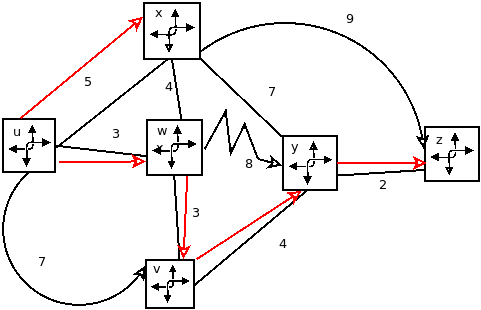
\includegraphics[width=.9\linewidth]{../img/dijkstraAlg.png}
\end{center}

\begin{center}
\begin{tabular}{rllllll}
 &  & D(v) & D(w) & D(x) & D(y) & D(z)\\
Step & N' & p(v) & p(w) & p(x) & p(y) & p(z)\\
\hline
0 & u & 7,u & \textbf{3,u} & 5,u & \bowtie & \bowtie\\
1 & uw & 6,w &  & \textbf{5,u} & 11,w & \\
2 & uwx & \textbf{6,w} &  &  & 11,w & 14,x\\
3 & uwxz &  &  &  & \textbf{10,v} & 14,x\\
4 & uwxvy &  &  &  &  & \textbf{12,y}\\
5 & uwxvyz &  &  &  &  & \\
\hline
\end{tabular}
\end{center}

\textbf{Notes}
\begin{itemize}
\item Construct shortest path by tracing predecessor nodes
\item Ties can exist (can be broken arbitrarily)
\end{itemize}

\textbf{Resuslting shortest-path tree from u:}
\begin{center}
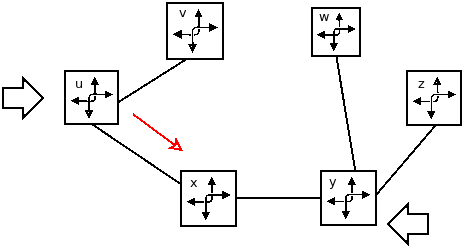
\includegraphics[width=.9\linewidth]{../img/resultShortPath.png}
\end{center}

Resulting forwarding table in u:

\begin{center}
\begin{tabular}{ll}
destination & link\\
\hline
v & (u.v)\\
x & (u.x)\\
y & (u.x)\\
w & (u.x)\\
z & (u.x)\\
\end{tabular}
\end{center}


\subsubsection{Bellman-Ford (Distance Vector Algorithm)}
\label{sec:org30f01de}

\begin{center}
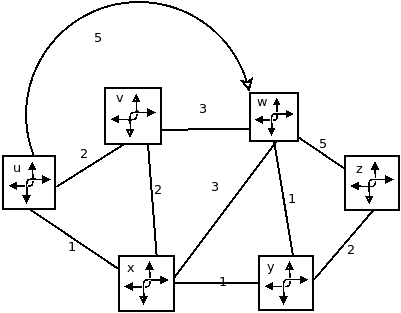
\includegraphics[width=.9\linewidth]{../img/graphAbstraction.png}
\end{center}

\begin{itemize}
\item Clearly, dv(z) = 5, dx(z) = 3, dw(z) = 3
\item B-F equation says: d\textsubscript{u} (z) = min \{ c(u, x) + dv(z), c(u, x) + dx(z),
c(u,w) + dw(z) \} = min \{ 2 + 5 , 1 + 3 , 5 + 3 \} = 4
\item From time-to-time, each node sends its own distance vector estimate
to neighbors
\item When x receives new DV estimate from neighbor, it updates its own DV
using B-F equation: D\textsubscript{x} (y) \(\leftarrow\) min\textsubscript{v} \{ c(x, v) + D\textsubscript{v}(y) \}
for each node y E N
\item Under minor, natural conditions, the estimate Dx(y) converge to the
actual least cost dx(y)
\end{itemize}


\subsubsection{Comparison of LS \& DV Algorithms}
\label{sec:org7388c44}

\textbf{Message Complexity}
\begin{itemize}
\item LS: With n nodes, E links, O(nE) msgs sent
\item DV: Exchange between neighbors only 
\begin{itemize}
\item Convergence time varies
\end{itemize}
\end{itemize}

\textbf{Robustness} What happens if router malfunctions?
\begin{itemize}
\item LS: 
\begin{itemize}
\item Node can advertise incorrect \emph{link cost}
\item Each node computes only its own table
\end{itemize}

\item DV:
\begin{itemize}
\item DV node can advertise incorrect \emph{path cost}
\item Each node's table used by others error propagates through network
\end{itemize}
\end{itemize}

\textbf{Domain}
\begin{itemize}
\item DV => local networks
\item LS => Global networks
\end{itemize}

\textbf{Speed of convergence}
\begin{itemize}
\item LS: O(n2) algorithm requires O(nE) msgs
\begin{itemize}
\item may have oscillations
\end{itemize}
\item DV: convergence time varies
\begin{itemize}
\item may be routing loops
\item count-to-infinity problem
\end{itemize}
\end{itemize}

\textbf{Hierarchical Routing}
\begin{itemize}
\item Routing study so far - idealization
\item All routers identical
\item Network "flat"
\end{itemize}
\ldots{} Not true in practice!

Scale: with 600 million destinations:
\begin{itemize}
\item Can't store all destinations in routing tables
\item Routing table exchange would swamp links
\end{itemize}

Administrative autonomy
\begin{itemize}
\item Internet = network of networkds
\item Each network admin may want to control routing in its own network
\end{itemize}


\subsection{Routing in the Internet}
\label{sec:orgebeda86}

\subsubsection{Autonomous systems}
\label{sec:orgd5fa9e8}

\begin{itemize}
\item Aggregate routers into regions \emph{"Autonomous Systems" (AS)}

\item Routers in some AS run some routing protocol
\begin{itemize}
\item \emph{"intra-AS" routing} protocol

\item Routers in different AS can be different intra-AS routing protocol
\end{itemize}

\item Gateway router:
\begin{itemize}
\item Routers in different AS can run different intra-AS routing protocol
\item Has link to router in another AS
\end{itemize}
\end{itemize}

\begin{center}
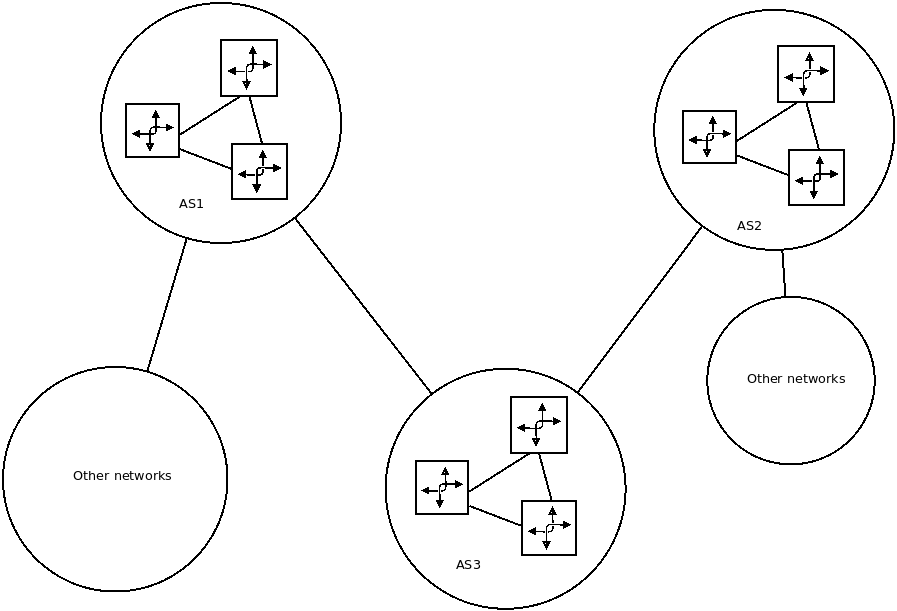
\includegraphics[width=.9\linewidth]{../img/autonomousSystems.png}
\end{center}

\begin{itemize}
\item Suppose router in AS1 receives datagram destined outside of AS1
\item AS1 must:
\begin{enumerate}
\item Learn which destinations are reachable through AS2, which through
AS3
\item Propagate this reachability info to all routers in AS1
\end{enumerate}
\end{itemize}


\subsubsection{Intra-AS routing}
\label{sec:orgd9548e1}
\begin{itemize}
\item Also known as interior gateway protocols (IGP)
\item Most common intra-AS routing protocols:
\begin{itemize}
\item RIP: Routing Information Protocol
\item OSPF: Open Shortest Path First
\item IGRP: Interior Gateway Routing Protocol (Cisco Proprietary)
\end{itemize}
\end{itemize}

\subsubsection{RIP (Routing Information Protocol)}
\label{sec:orgccc962e}
\begin{itemize}
\item Included in BSD-Linux distribution in 1982
\item Distance vector algorithm
\begin{itemize}
\item distance metric: number of hops ( max = 15 hops), each link has
cost 1
\item DVs exchanged with neighbors every 30 seconds in response message
(aka advertisement)
\item Each advertisement: lists up to 25 destination subnets (in IP
addressing sense)
\end{itemize}

\item If no advertisement heard after 180 seconds, neighbor link declared
dead
\begin{itemize}
\item Routes via neighbor invalidated

\item new advertisements sent to neighbors

\item neighboers in turn send out new advertisements (if tables changed)
\end{itemize}
\item Link failure info quickly propagates to entire net
\item Poison reverse used to precent ping-pong loops (infinite distance =
16 hops)
\end{itemize}

\subsubsection{Open Shortest Path First}
\label{sec:org91e8913}
\begin{itemize}
\item "Open" source
\item Uses link state algorithm
\begin{itemize}
\item LS packet dissemination
\item Topology map at each node
\item Route computation using Dijkstra's algorithm
\end{itemize}
\item OSPF advertisement carries one entry per neighbor
\item Advertisements flooded to entire AS 
\begin{itemize}
\item Carried in OSPF message directly over IP (rather than TCP or UDP)
\end{itemize}
\item Security: all OSPF messages authenticated (to prevent malicious intrusion)
\item Multiple some-cost paths allowed (only one in RIP)
\item For each link, multiple cost metrics for different ToS (e.g.:
satellite link cost set "low" for best effore ToS; high for real
time ToS
\item Integrated uni and multicast support 
\begin{itemize}
\item Multicast OSPF (MOSPF) uses some topology database as OSPF
\end{itemize}
\item Hierarchical OSPF in large domains
\end{itemize}


\subsubsection{Hierarchical OSPF}
\label{sec:orgd8a8ffa}

\begin{center}
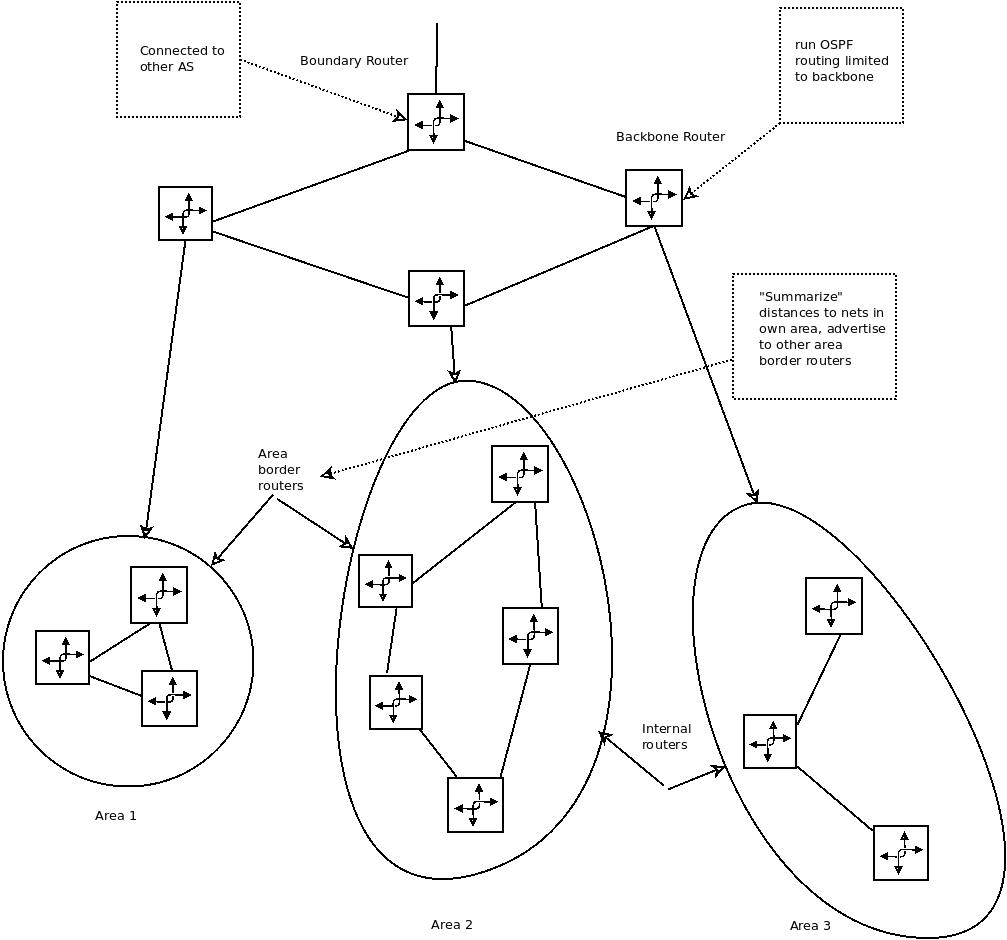
\includegraphics[width=.9\linewidth]{../img/ospf.png}
\end{center}

\begin{itemize}
\item Two-level hierarchy: local area, backbone
\begin{itemize}
\item Link-state advertisements only in area
\item Each node has detailed area topology; only know direction
(shortest path) to nets in other areas
\end{itemize}
\end{itemize}

\subsubsection{Border Gateway Protocol (BGP)}
\label{sec:orgd007fd4}
\begin{itemize}
\item De Facto inter-domain routing protocol 
\begin{itemize}
\item "glue that holds the internet together"
\end{itemize}

\item BGP provides each AS a means to:
\begin{itemize}
\item eBGP: obtain subnet reachability information from neighboring ASs
\item iBGP: propagate reachability information to all AS-internal routers
\item Determins "good" routes to other networks based on reachability
information and policy
\end{itemize}
\item Allows subnet to advertise its existence to rest of internet: "I Am
Here!"
\end{itemize}

\subsubsection{Why different routing?}
\label{sec:org9b88e26}

\begin{center}
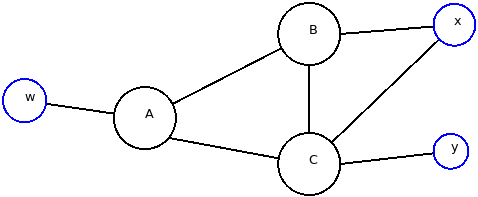
\includegraphics[width=.9\linewidth]{../img/bgp.png}
\end{center}

\begin{itemize}
\item A, B, C are provider networks
\item x, w, y are customer (of provider networks)
\item x is \emph{dual-homed}: attached to two networks
\begin{itemize}
\item x does not want to route B via X to C
\item \ldots{} so x will not advertise to B a route to C
\end{itemize}
\end{itemize}

\textbf{Policy}
\begin{itemize}
\item Inter-AS: admin wants to control over how its traffic routed, who
routes through its net
\item intra-AS: single admin, so no policy decisions needed
\end{itemize}

\textbf{Scale}
\begin{itemize}
\item hierarchical routing saves table size, reduced update traffic
\end{itemize}

\textbf{Performance}
\begin{itemize}
\item intra-AS: can focus on performance
\item inter-AS: policy may dominate over performance
\end{itemize}

\subsubsection{Broadcast \& Multitask routing}
\label{sec:org5d68de5}
\begin{itemize}
\item Deliver packets from source to all other nodes
\item Source duplication is ineffecient
\end{itemize}

\begin{center}
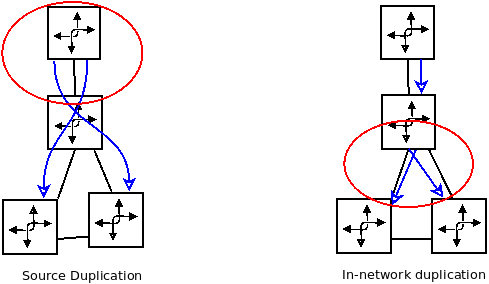
\includegraphics[width=.9\linewidth]{../img/broadcastMultitask.png}
\end{center}

\begin{itemize}
\item Flooding: When node receives broadcast packet, sends copy to all
neighbors
\begin{itemize}
\item Problems: cycles \& broadcast storm
\end{itemize}
\item Controlled flooding: node only broadcasts packet if it hasn't
broadcast same packet before
\begin{itemize}
\item Node keeps track of packet ids already broadcasted
\item Or reverse path forwarding (RPF): only forwarded packet if it
arrived on shortest path between node and source
\end{itemize}

\item Spanning tree:
\begin{itemize}
\item No redundent packets by any node

\item First construct spanning tree

\item Nodes then forwarded/make copies only along spanning tree
\end{itemize}
\end{itemize}

\begin{center}
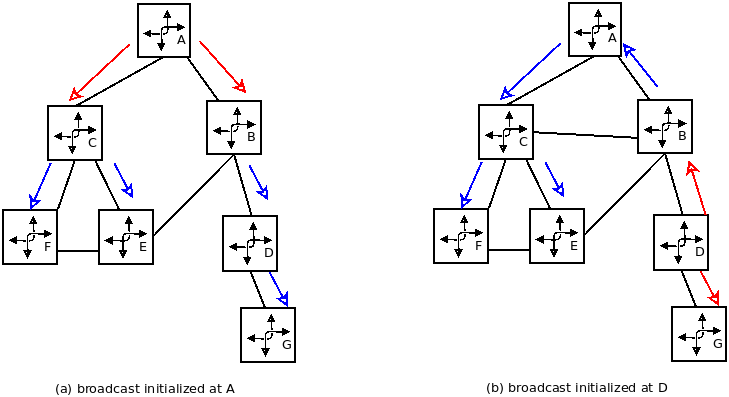
\includegraphics[width=.9\linewidth]{../img/spanningTree.png}
\end{center}

\subsubsection{Multicast routing}
\label{sec:org7831e03}
\begin{itemize}
\item Delivers to multiple but not all computers in the network
\end{itemize}
\end{document}
